\documentclass[]{article}
\usepackage{lmodern}
\usepackage{amssymb,amsmath}
\usepackage{ifxetex,ifluatex}
\usepackage{fixltx2e} % provides \textsubscript
\ifnum 0\ifxetex 1\fi\ifluatex 1\fi=0 % if pdftex
  \usepackage[T1]{fontenc}
  \usepackage[utf8]{inputenc}
\else % if luatex or xelatex
  \ifxetex
    \usepackage{mathspec}
  \else
    \usepackage{fontspec}
  \fi
  \defaultfontfeatures{Ligatures=TeX,Scale=MatchLowercase}
\fi
% use upquote if available, for straight quotes in verbatim environments
\IfFileExists{upquote.sty}{\usepackage{upquote}}{}
% use microtype if available
\IfFileExists{microtype.sty}{%
\usepackage{microtype}
\UseMicrotypeSet[protrusion]{basicmath} % disable protrusion for tt fonts
}{}
\usepackage[margin=1in]{geometry}
\usepackage{hyperref}
\hypersetup{unicode=true,
            pdftitle={Temperature dependence of biomass and ecosystem function depend on species interactions. Supplementary File 3: Zooplankton figures and tables.},
            pdfborder={0 0 0},
            breaklinks=true}
\urlstyle{same}  % don't use monospace font for urls
\usepackage{longtable,booktabs}
\usepackage{graphicx,grffile}
\makeatletter
\def\maxwidth{\ifdim\Gin@nat@width>\linewidth\linewidth\else\Gin@nat@width\fi}
\def\maxheight{\ifdim\Gin@nat@height>\textheight\textheight\else\Gin@nat@height\fi}
\makeatother
% Scale images if necessary, so that they will not overflow the page
% margins by default, and it is still possible to overwrite the defaults
% using explicit options in \includegraphics[width, height, ...]{}
\setkeys{Gin}{width=\maxwidth,height=\maxheight,keepaspectratio}
\IfFileExists{parskip.sty}{%
\usepackage{parskip}
}{% else
\setlength{\parindent}{0pt}
\setlength{\parskip}{6pt plus 2pt minus 1pt}
}
\setlength{\emergencystretch}{3em}  % prevent overfull lines
\providecommand{\tightlist}{%
  \setlength{\itemsep}{0pt}\setlength{\parskip}{0pt}}
\setcounter{secnumdepth}{0}
% Redefines (sub)paragraphs to behave more like sections
\ifx\paragraph\undefined\else
\let\oldparagraph\paragraph
\renewcommand{\paragraph}[1]{\oldparagraph{#1}\mbox{}}
\fi
\ifx\subparagraph\undefined\else
\let\oldsubparagraph\subparagraph
\renewcommand{\subparagraph}[1]{\oldsubparagraph{#1}\mbox{}}
\fi

%%% Use protect on footnotes to avoid problems with footnotes in titles
\let\rmarkdownfootnote\footnote%
\def\footnote{\protect\rmarkdownfootnote}

%%% Change title format to be more compact
\usepackage{titling}

% Create subtitle command for use in maketitle
\providecommand{\subtitle}[1]{
  \posttitle{
    \begin{center}\large#1\end{center}
    }
}

\setlength{\droptitle}{-2em}

  \title{Temperature dependence of biomass and ecosystem function depend on
species interactions. Supplementary File 3: Zooplankton figures and
tables.}
    \pretitle{\vspace{\droptitle}\centering\huge}
  \posttitle{\par}
    \author{}
    \preauthor{}\postauthor{}
    \date{}
    \predate{}\postdate{}
  

\begin{document}
\maketitle

\paragraph{Section S3.1: Zooplankton Abundance data over whole
experiment}\label{section-s3.1-zooplankton-abundance-data-over-whole-experiment}

Figure S3. 1: Abundance of zooplankton (Number / 10L) over all tanks and
weeks.

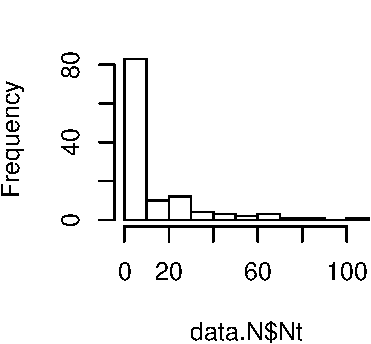
\includegraphics{Garzke_zooplankton_files/figure-latex/Fig_S3.1: Histogram ZP Abundance-1.pdf}
\includegraphics{Garzke_zooplankton_files/figure-latex/Fig_S3.1: Histogram ZP Abundance-2.pdf}

Figure S3. 2: Residual plot for linear model of abundance with normally
distributed errors

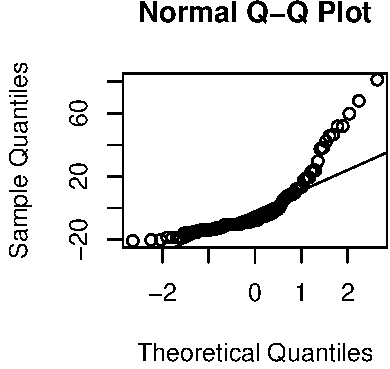
\includegraphics{Garzke_zooplankton_files/figure-latex/resid_plot_lm-1.pdf}

\section{april 2019 b}\label{april-2019-b}

\includegraphics{Garzke_zooplankton_files/figure-latex/log density-1.pdf}

Table S3. 1: Model selection results for zooplankton abundance, with
1\textbar{}Tank as a random effect. Model terms are: intercept (Int),
Temperature - weekly average (Tw), trophic treatment (TL), statistical
estimates

\begin{longtable}[]{@{}lrrllrrrrr@{}}
\toprule
& Int & T\textsubscript{wj} & Z\textsubscript{j} & & df & logLik & AICc
& d & w\tabularnewline
\midrule
\endhead
m1c & 1.56 & NA & NA & NA & 3 & -218.17 & 442.56 & 0.00 &
0.2179787\tabularnewline
m1 & 1.82 & 0.78 & + & + & 6 & -214.92 & 442.58 & 0.02 &
0.2157004\tabularnewline
m1b & 1.56 & 0.66 & NA & NA & 4 & -217.17 & 442.69 & 0.14 &
0.2034743\tabularnewline
m1d & 1.82 & 0.74 & + & NA & 5 & -216.18 & 442.89 & 0.34 &
0.1843232\tabularnewline
m1a & 1.81 & NA & + & NA & 4 & -217.30 & 442.96 & 0.40 &
0.1785234\tabularnewline
\bottomrule
\end{longtable}

\section{april 2019}\label{april-2019}

Figure S3. 3: Total Zooplankton abundance and modeled temperature
dependence from negative binomial regression

\includegraphics{Garzke_zooplankton_files/figure-latex/N_plot-1.pdf}

\paragraph{}\label{section}

\paragraph{}\label{section-1}

\paragraph{}\label{section-2}

\subsubsection{Section S3.2: Daphnia and
Copepods}\label{section-s3.2-daphnia-and-copepods}

Figure S3. 4: Abundance of Daphnia and Copepods (Number / 10L) over all
tanks and weeks.

\includegraphics{Garzke_zooplankton_files/figure-latex/Daphnia_abundance-1.pdf}
\includegraphics{Garzke_zooplankton_files/figure-latex/Daphnia_abundance-2.pdf}

\includegraphics{Garzke_zooplankton_files/figure-latex/log Daphnia density-1.pdf}

Table S3. 2: Daphnia abundance model selection results for Poisson
regression. Model terms are: intercept (Int), trophic treatment (TL),
Temperature - weekly average (Tw), and statistical estimates

\begin{longtable}[]{@{}lrrllrrrrr@{}}
\toprule
& Int & T\textsubscript{wj} & Z\textsubscript{j} &
T\textsubscript{wj}*Z\textsubscript{j} & df & logLik & AICc & d &
w\tabularnewline
\midrule
\endhead
m1Da & 0.40 & NA & + & NA & 4 & -75.77 & 159.89 & 0.00 &
0.40457193\tabularnewline
m1Dc & 0.28 & NA & NA & NA & 3 & -76.88 & 159.96 & 0.07 &
0.39089048\tabularnewline
m1Dd & 0.40 & 0.15 & + & NA & 5 & -76.19 & 162.92 & 3.02 &
0.08923334\tabularnewline
m1Db & 0.28 & 0.11 & NA & NA & 4 & -77.35 & 163.05 & 3.15 &
0.08366792\tabularnewline
m1D & 0.40 & 0.20 & + & + & 6 & -76.12 & 164.99 & 5.10 &
0.03163634\tabularnewline
\bottomrule
\end{longtable}

Table S3. 3: Daphnia abundance model coefficients

\includegraphics{Garzke_zooplankton_files/figure-latex/log Copepod density-1.pdf}

Table S3. 4: Copepod abundance model selection results for Poisson
regression. Model terms are: intercept (Int), trophic treatment (TL),
Temperature - weekly average (Tw), temperature - expt average (Tt),
interaction terms and statistical estimates

\begin{longtable}[]{@{}lrrllrrrrr@{}}
\toprule
& Int & T\textsubscript{wj} & Z\textsubscript{j} &
T\textsubscript{wj}*Z\textsubscript{j} & df & logLik & AICc & d &
w\tabularnewline
\midrule
\endhead
m1Cb & 1.16 & 1.20 & NA & NA & 4 & -199.71 & 407.77 & 0.00 &
0.54916077\tabularnewline
m1C & 1.19 & 1.32 & + & + & 6 & -198.88 & 410.51 & 2.74 &
0.13941921\tabularnewline
m1Cd & 1.19 & 1.21 & + & NA & 5 & -200.01 & 410.54 & 2.77 &
0.13725194\tabularnewline
m1Cc & 1.16 & NA & NA & NA & 3 & -202.17 & 410.54 & 2.78 &
0.13699614\tabularnewline
m1Ca & 1.16 & NA & + & NA & 4 & -202.40 & 413.15 & 5.39 &
0.03717194\tabularnewline
\bottomrule
\end{longtable}

Table S3. 5: Copepod abundance model coefficients

\begin{verbatim}
## pdf 
##   2
\end{verbatim}


\end{document}
